%! Author = Philipp Emmenegger
%! Date = 10/06/2021

\section{Introduction}
\textbf{Formal Methods}
\begin{itemize}
    \item Application of theoretical computer science fundamentals
    \item Logic calculi
    \item Formal languages
    \item Automata theory
    \item Program semantics
    \item Type systems
    \item Algebraic data types
\end{itemize}

\textbf{Formal Language}
\begin{itemize}
    \item Set of strings of symbols
    \item Constrained by specific rules
    \item Programming languages
    \item Usage: Specify, invent, transform, analyse, verify, reason about programming languages
    \item Informal: living natural languages
\end{itemize}

\subsection{Execution-based vs. Rule-based thinking}
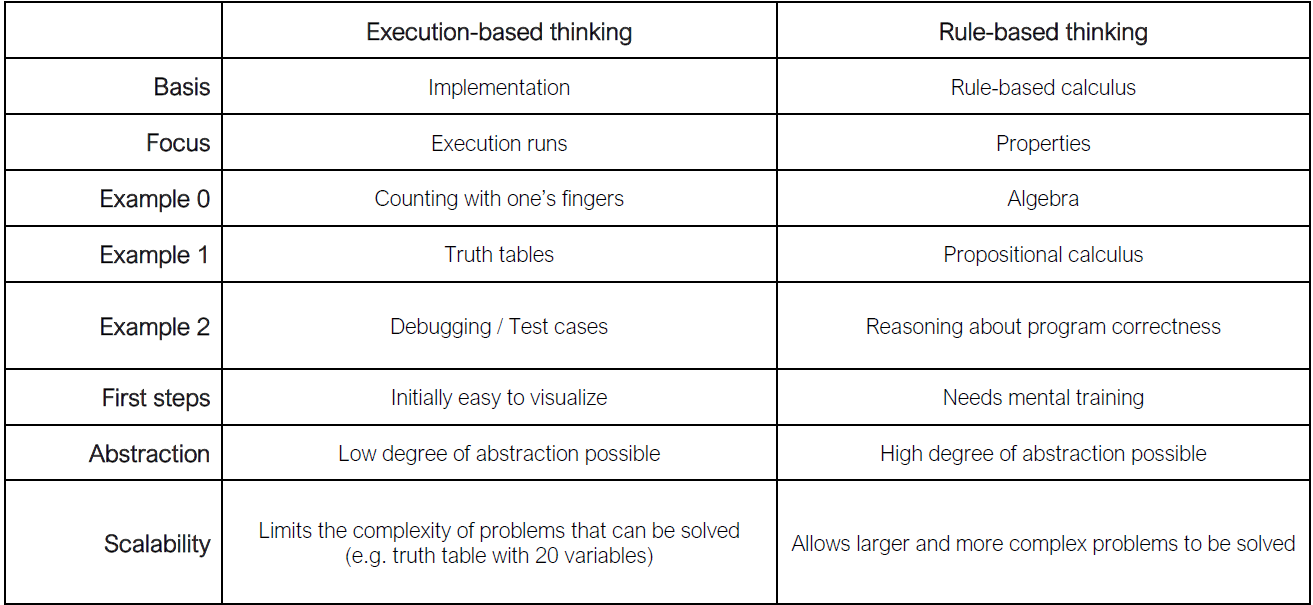
\includegraphics[width=\linewidth]{../img/execution_rule_thinking.png}

\section{Programming Paradigms}
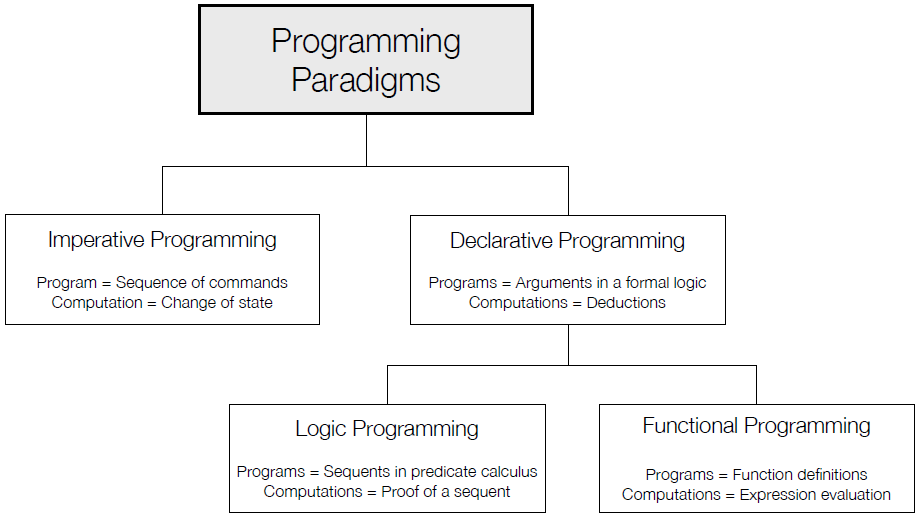
\includegraphics[width=\linewidth]{../img/programming_paradigms.png}
\subsection{Imperative}
\begin{itemize}
    \item Befehlend
    \item Focuses on \textbf{how} a program operates
    \item Commands change a program's state
\end{itemize}
\textbf{Common building blocks:}
\begin{itemize}
    \item Assignment: $x := x + 1$
    \item Sequential composition: $(... ; ...)$
    \item Conditional execution: $(if ... then ... else)$
    \item Repetition: $(while ... do ...)$ / $(goto ...)$
\end{itemize}
\subsubsection{Von Neumann architecture}
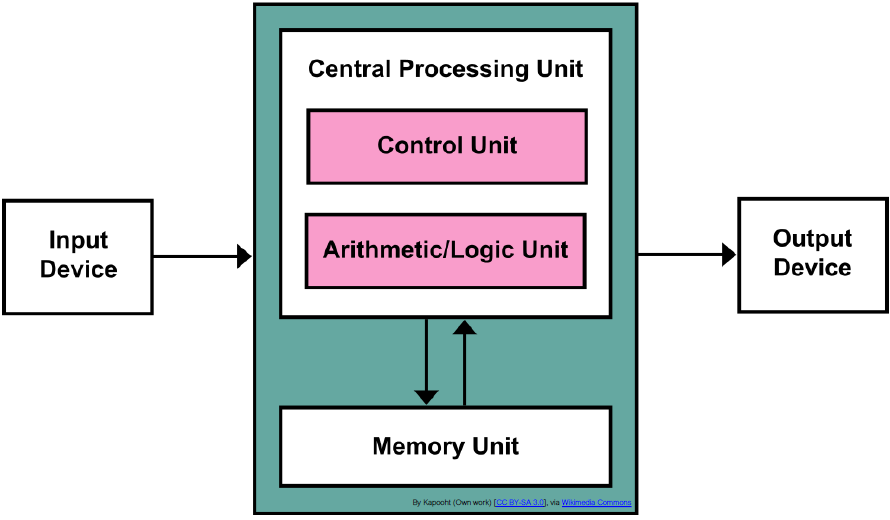
\includegraphics[width=0.7\linewidth]{../img/imperative_programming.png}\\

\subsection{Declarative}
\begin{itemize}
    \item Expresses the logic of a computation without describing its control flow
    \item Describes \textbf{what} the program should accomplish
    \item \textbf{how} - left to the language's implementation
    \item eliminates / minimises side effects
\end{itemize}
\textbf{Examples:}
\begin{itemize}
    \item Spreadsheets
    \item Regular expressions
    \item Query languages
    \item Functional programming languages
    \item Logic programming
\end{itemize}

\section{Functional Programming Introduction}
\textbf{Basic Features}
\begin{itemize}
    \item Referential transparency
    \item Functions as first-class citizens
    \item Higher-order functions
    \item Algebraic data types
    \item Pattern matching
    \item Recursion
    \item Types \& type inference
    \item Haskell specific: Type classes, Functors, Applicatives, Monads
\end{itemize}
\textbf{What is FP?}
\begin{itemize}
    \item Declarative programming paradigm
    \item Foundation: Chruch's Lambda calculus
    \item Pure: No (or controlled) mutable state
    \item Pure: Expressions are by default side effect free
\end{itemize}

\textbf{Why functions?}
\begin{itemize}
    \item Simple concept and properties
    \item High level of abstraction possible
    \item Powerful reasoning more easily possible
\end{itemize}

\textbf{Why use FP?}
\begin{itemize}
    \item Easier to reason about
    \item Easier to write
    \item Easier to get right
\end{itemize}

\subsection{No Mutable State}
\begin{itemize}
    \item Referential Transparency: WYSIWYG for programmers
    \item $f(x)$ only depends on the def. of $f$ and the value of $x$
    \item \textbf{No} mutable variables
    \item \textbf{No} assignments
    \item \textbf{No} imperative control structures
    \item All data structures are immutable
\end{itemize}
\textbf{Problem with mutable state}
\begin{itemize}
    \item Every statement can potentially change the underlying state of the program
    \item Executions of a statement can depend on previously executed statements
\end{itemize}

\subsection{Functions are first-class Citizens}
\begin{itemize}
    \item just like any other values: $1, true$
    \item Can be anonymous: $(\lambda x . x + 1)$
    \item Can be input/output to other functions
    \item Can be composed in powerful ways $f o g$
\end{itemize}

\subsection{More FP in the future}
\begin{itemize}
    \item Increased expectations on reliability of software
    \item Increased demands on scalability, complexity, performance
    \item FP can surpass the limitations of the mainstream
    \item FP is an active area of applied research
    \item Increased adoption of FP features in mainstream languages (generics)
\end{itemize}
\columnbreak





